%% bare_conf.tex
%% V1.4
%% 2012/12/27
%% by Michael Shell
%% See:
%% http://www.michaelshell.org/
%% for current contact information.
%%
%% This is a skeleton file demonstrating the use of IEEEtran.cls
%% (requires IEEEtran.cls version 1.8 or later) with an IEEE conference paper.
%%
%% Support sites:
%% http://www.michaelshell.org/tex/ieeetran/
%% http://www.ctan.org/tex-archive/macros/latex/contrib/IEEEtran/
%% and
%% http://www.ieee.org/

%%*************************************************************************
%% Legal Notice:
%% This code is offered as-is without any warranty either expressed or
%% implied; without even the implied warranty of MERCHANTABILITY or
%% FITNESS FOR A PARTICULAR PURPOSE! 
%% User assumes all risk.
%% In no event shall IEEE or any contributor to this code be liable for
%% any damages or losses, including, but not limited to, incidental,
%% consequential, or any other damages, resulting from the use or misuse
%% of any information contained here.
%%
%% All comments are the opinions of their respective authors and are not
%% necessarily endorsed by the IEEE.
%%
%% This work is distributed under the LaTeX Project Public License (LPPL)
%% ( http://www.latex-project.org/ ) version 1.3, and may be freely used,
%% distributed and modified. A copy of the LPPL, version 1.3, is included
%% in the base LaTeX documentation of all distributions of LaTeX released
%% 2003/12/01 or later.
%% Retain all contribution notices and credits.
%% ** Modified files should be clearly indicated as such, including  **
%% ** renaming them and changing author support contact information. **
%%
%% File list of work: IEEEtran.cls, IEEEtran_HOWTO.pdf, bare_adv.tex,
%%                    bare_conf.tex, bare_jrnl.tex, bare_jrnl_compsoc.tex,
%%                    bare_jrnl_transmag.tex
%%*************************************************************************

% *** Authors should verify (and, if needed, correct) their LaTeX system  ***
% *** with the testflow diagnostic prior to trusting their LaTeX platform ***
% *** with production work. IEEE's font choices can trigger bugs that do  ***
% *** not appear when using other class files.                            ***
% The testflow support page is at:
% http://www.michaelshell.org/tex/testflow/



% Note that the a4paper option is mainly intended so that authors in
% countries using A4 can easily print to A4 and see how their papers will
% look in print - the typesetting of the document will not typically be
% affected with changes in paper size (but the bottom and side margins will).
% Use the testflow package mentioned above to verify correct handling of
% both paper sizes by the user's LaTeX system.
%
% Also note that the "draftcls" or "draftclsnofoot", not "draft", option
% should be used if it is desired that the figures are to be displayed in
% draft mode.
%
\documentclass[conference]{IEEEtran}
% Add the compsoc option for Computer Society conferences.
%
% If IEEEtran.cls has not been installed into the LaTeX system files,
% manually specify the path to it like:
% \documentclass[conference]{../sty/IEEEtran}



% Some very useful LaTeX packages include:
% (uncomment the ones you want to load)


% *** MISC UTILITY PACKAGES ***
%
\usepackage[utf8]{inputenc}
\usepackage[ngerman]{babel}
%\usepackage{ifpdf}
% Heiko Oberdiek's ifpdf.sty is very useful if you need conditional
% compilation based on whether the output is pdf or dvi.
% usage:
% \ifpdf
%   % pdf code
% \else
%   % dvi code
% \fi
% The latest version of ifpdf.sty can be obtained from:
% http://www.ctan.org/tex-archive/macros/latex/contrib/oberdiek/
% Also, note that IEEEtran.cls V1.7 and later provides a builtin
% \ifCLASSINFOpdf conditional that works the same way.
% When switching from latex to pdflatex and vice-versa, the compiler may
% have to be run twice to clear warning/error messages.






% *** CITATION PACKAGES ***
%
\usepackage{cite}
% cite.sty was written by Donald Arseneau
% V1.6 and later of IEEEtran pre-defines the format of the cite.sty package
% \cite{} output to follow that of IEEE. Loading the cite package will
% result in citation numbers being automatically sorted and properly
% "compressed/ranged". e.g., [1], [9], [2], [7], [5], [6] without using
% cite.sty will become [1], [2], [5]--[7], [9] using cite.sty. cite.sty's
% \cite will automatically add leading space, if needed. Use cite.sty's
% noadjust option (cite.sty V3.8 and later) if you want to turn this off
% such as if a citation ever needs to be enclosed in parenthesis.
% cite.sty is already installed on most LaTeX systems. Be sure and use
% version 4.0 (2003-05-27) and later if using hyperref.sty. cite.sty does
% not currently provide for hyperlinked citations.
% The latest version can be obtained at:
% http://www.ctan.org/tex-archive/macros/latex/contrib/cite/
% The documentation is contained in the cite.sty file itself.

\usepackage{hyperref}



% *** GRAPHICS RELATED PACKAGES ***
%
\ifCLASSINFOpdf
  \usepackage[pdftex]{graphicx}
  % declare the path(s) where your graphic files are
  % \graphicspath{{../pdf/}{../jpeg/}}
  % and their extensions so you won't have to specify these with
  % every instance of \includegraphics
  % \DeclareGraphicsExtensions{.pdf,.jpeg,.png}
\else
  % or other class option (dvipsone, dvipdf, if not using dvips). graphicx
  % will default to the driver specified in the system graphics.cfg if no
  % driver is specified.
  \usepackage[dvips]{graphicx}
  % declare the path(s) where your graphic files are
  % \graphicspath{{../eps/}}
  % and their extensions so you won't have to specify these with
  % every instance of \includegraphics
  % \DeclareGraphicsExtensions{.eps}
\fi
% graphicx was written by David Carlisle and Sebastian Rahtz. It is
% required if you want graphics, photos, etc. graphicx.sty is already
% installed on most LaTeX systems. The latest version and documentation
% can be obtained at: 
% http://www.ctan.org/tex-archive/macros/latex/required/graphics/
% Another good source of documentation is "Using Imported Graphics in
% LaTeX2e" by Keith Reckdahl which can be found at:
% http://www.ctan.org/tex-archive/info/epslatex/
%
% latex, and pdflatex in dvi mode, support graphics in encapsulated
% postscript (.eps) format. pdflatex in pdf mode supports graphics
% in .pdf, .jpeg, .png and .mps (metapost) formats. Users should ensure
% that all non-photo figures use a vector format (.eps, .pdf, .mps) and
% not a bitmapped formats (.jpeg, .png). IEEE frowns on bitmapped formats
% which can result in "jaggedy"/blurry rendering of lines and letters as
% well as large increases in file sizes.
%
% You can find documentation about the pdfTeX application at:
% http://www.tug.org/applications/pdftex

\usepackage{fixltx2e}



% *** MATH PACKAGES ***
%
%\usepackage[cmex10]{amsmath}
% A popular package from the American Mathematical Society that provides
% many useful and powerful commands for dealing with mathematics. If using
% it, be sure to load this package with the cmex10 option to ensure that
% only type 1 fonts will utilized at all point sizes. Without this option,
% it is possible that some math symbols, particularly those within
% footnotes, will be rendered in bitmap form which will result in a
% document that can not be IEEE Xplore compliant!
%
% Also, note that the amsmath package sets \interdisplaylinepenalty to 10000
% thus preventing page breaks from occurring within multiline equations. Use:
%\interdisplaylinepenalty=2500
% after loading amsmath to restore such page breaks as IEEEtran.cls normally
% does. amsmath.sty is already installed on most LaTeX systems. The latest
% version and documentation can be obtained at:
% http://www.ctan.org/tex-archive/macros/latex/required/amslatex/math/





% *** SPECIALIZED LIST PACKAGES ***
%
%\usepackage{algorithmic}
% algorithmic.sty was written by Peter Williams and Rogerio Brito.
% This package provides an algorithmic environment fo describing algorithms.
% You can use the algorithmic environment in-text or within a figure
% environment to provide for a floating algorithm. Do NOT use the algorithm
% floating environment provided by algorithm.sty (by the same authors) or
% algorithm2e.sty (by Christophe Fiorio) as IEEE does not use dedicated
% algorithm float types and packages that provide these will not provide
% correct IEEE style captions. The latest version and documentation of
% algorithmic.sty can be obtained at:
% http://www.ctan.org/tex-archive/macros/latex/contrib/algorithms/
% There is also a support site at:
% http://algorithms.berlios.de/index.html
% Also of interest may be the (relatively newer and more customizable)
% algorithmicx.sty package by Szasz Janos:
% http://www.ctan.org/tex-archive/macros/latex/contrib/algorithmicx/




% *** ALIGNMENT PACKAGES ***
%
%\usepackage{array}
% Frank Mittelbach's and David Carlisle's array.sty patches and improves
% the standard LaTeX2e array and tabular environments to provide better
% appearance and additional user controls. As the default LaTeX2e table
% generation code is lacking to the point of almost being broken with
% respect to the quality of the end results, all users are strongly
% advised to use an enhanced (at the very least that provided by array.sty)
% set of table tools. array.sty is already installed on most systems. The
% latest version and documentation can be obtained at:
% http://www.ctan.org/tex-archive/macros/latex/required/tools/


% IEEEtran contains the IEEEeqnarray family of commands that can be used to
% generate multiline equations as well as matrices, tables, etc., of high
% quality.




% *** SUBFIGURE PACKAGES ***
%\ifCLASSOPTIONcompsoc
%  \usepackage[caption=false,font=normalsize,labelfont=sf,textfont=sf]{subfig}
%\else
%  \usepackage[caption=false,font=footnotesize]{subfig}
%\fi
% subfig.sty, written by Steven Douglas Cochran, is the modern replacement
% for subfigure.sty, the latter of which is no longer maintained and is
% incompatible with some LaTeX packages including fixltx2e. However,
% subfig.sty requires and automatically loads Axel Sommerfeldt's caption.sty
% which will override IEEEtran.cls' handling of captions and this will result
% in non-IEEE style figure/table captions. To prevent this problem, be sure
% and invoke subfig.sty's "caption=false" package option (available since
% subfig.sty version 1.3, 2005/06/28) as this is will preserve IEEEtran.cls
% handling of captions.	
% Note that the Computer Society format requires a larger sans serif font
% than the serif footnote size font used in traditional IEEE formatting
% and thus the need to invoke different subfig.sty package options depending
% on whether compsoc mode has been enabled.
%
% The latest version and documentation of subfig.sty can be obtained at:
% http://www.ctan.org/tex-archive/macros/latex/contrib/subfig/




% *** FLOAT PACKAGES ***
%
%\usepackage{fixltx2e}
% fixltx2e, the successor to the earlier fix2col.sty, was written by
% Frank Mittelbach and David Carlisle. This package corrects a few problems
% in the LaTeX2e kernel, the most notable of which is that in current
% LaTeX2e releases, the ordering of single and double column floats is not
% guaranteed to be preserved. Thus, an unpatched LaTeX2e can allow a
% single column figure to be placed prior to an earlier double column
% figure. The latest version and documentation can be found at:
% http://www.ctan.org/tex-archive/macros/latex/base/


%\usepackage{stfloats}
% stfloats.sty was written by Sigitas Tolusis. This package gives LaTeX2e
% the ability to do double column floats at the bottom of the page as well
% as the top. (e.g., "\begin{figure*}[!b]" is not normally possible in
% LaTeX2e). It also provides a command:
%\fnbelowfloat
% to enable the placement of footnotes below bottom floats (the standard
% LaTeX2e kernel puts them above bottom floats). This is an invasive package
% which rewrites many portions of the LaTeX2e float routines. It may not work
% with other packages that modify the LaTeX2e float routines. The latest
% version and documentation can be obtained at:
% http://www.ctan.org/tex-archive/macros/latex/contrib/sttools/
% Do not use the stfloats baselinefloat ability as IEEE does not allow
% \baselineskip to stretch. Authors submitting work to the IEEE should note
% that IEEE rarely uses double column equations and that authors should try
% to avoid such use. Do not be tempted to use the cuted.sty or midfloat.sty
% packages (also by Sigitas Tolusis) as IEEE does not format its papers in
% such ways.
% Do not attempt to use stfloats with fixltx2e as they are incompatible.
% Instead, use Morten Hogholm'a dblfloatfix which combines the features
% of both fixltx2e and stfloats:
%
% \usepackage{dblfloatfix}
% The latest version can be found at:
% http://www.ctan.org/tex-archive/macros/latex/contrib/dblfloatfix/




% *** PDF, URL AND HYPERLINK PACKAGES ***
%
\usepackage{url}
% url.sty was written by Donald Arseneau. It provides better support for
% handling and breaking URLs. url.sty is already installed on most LaTeX
% systems. The latest version and documentation can be obtained at:
% http://www.ctan.org/tex-archive/macros/latex/contrib/url/
% Basically, \url{my_url_here}.




% *** Do not adjust lengths that control margins, column widths, etc. ***
% *** Do not use packages that alter fonts (such as pslatex).         ***
% There should be no need to do such things with IEEEtran.cls V1.6 and later.
% (Unless specifically asked to do so by the journal or conference you plan
% to submit to, of course. )

%\usepackage{subfigure}
%\usepackage{hyperref}
%%% Doc: ftp://tug.ctan.org/pub/tex-archive/.....ntrib/oberdiek/hypcap.pdf
% Links auf Gleitumgebungen springen nicht zur Beschriftung,
% sondern zum Anfang der Gleitumgebung
   %\usepackage[figure]{hypcap} 
   
\usepackage{subcaption}


% correct bad hyphenation here
\hyphenation{op-tical net-works semi-conduc-tor}

\begin{document}
%
% paper title
% can use linebreaks \\ within to get better formatting as desired
% Do not put math or special symbols in the title.
\title{Abschlussbericht - Computer Vision}


% author names and affiliations
% use a multiple column layout for up to three different
% affiliations
\author{\IEEEauthorblockN{Manuel Kosta}
\IEEEauthorblockA{Fakultät für Informatik\\
Otto-von-Guericke Universität\\
Magdeburg}
\and
\IEEEauthorblockN{Franz Kuntke}
\IEEEauthorblockA{Fakultät für Informatik\\
Otto-von-Guericke Universität\\
Magdeburg}}

% conference papers do not typically use \thanks and this command
% is locked out in conference mode. If really needed, such as for
% the acknowledgment of grants, issue a \IEEEoverridecommandlockouts
% after \documentclass

% for over three affiliations, or if they all won't fit within the width
% of the page, use this alternative format:
% 
%\author{\IEEEauthorblockN{Michael Shell\IEEEauthorrefmark{1},
%Homer Simpson\IEEEauthorrefmark{2},
%James Kirk\IEEEauthorrefmark{3}, 
%Montgomery Scott\IEEEauthorrefmark{3} and
%Eldon Tyrell\IEEEauthorrefmark{4}}
%\IEEEauthorblockA{\IEEEauthorrefmark{1}School of Electrical and Computer Engineering\\
%Georgia Institute of Technology,
%Atlanta, Georgia 30332--0250\\ Email: see http://www.michaelshell.org/contact.html}
%\IEEEauthorblockA{\IEEEauthorrefmark{2}Twentieth Century Fox, Springfield, USA\\
%Email: homer@thesimpsons.com}
%\IEEEauthorblockA{\IEEEauthorrefmark{3}Starfleet Academy, San Francisco, California 96678-2391\\
%Telephone: (800) 555--1212, Fax: (888) 555--1212}
%\IEEEauthorblockA{\IEEEauthorrefmark{4}Tyrell Inc., 123 Replicant Street, Los Angeles, California 90210--4321}}




% use for special paper notices
%\IEEEspecialpapernotice{(Invited Paper)}


% make the title area
\maketitle

% As a general rule, do not put math, special symbols or citations
% in the abstract
%\begin{abstract}
%The abstract goes here.
%\end{abstract}

% no keywords

% For peer review papers, you can put extra information on the cover
% page as needed:
% \ifCLASSOPTIONpeerreview
% \begin{center} \bfseries EDICS Category: 3-BBND \end{center}
% \fi
%
% For peerreview papers, this IEEEtran command inserts a page break and
% creates the second title. It will be ignored for other modes.
\IEEEpeerreviewmaketitle


\section{Einleitung}
% no \IEEEPARstart

%Hier kommt die Einleitung ...
 
%\hfill  28. Juni 2014


\subsection{Ziel des Projektes}
Im Rahmen des Projektes soll eine Bewegungssegmentierung implementiert werden, welche auf Verkehrsszenen mit starrer Kamera angewandt wird. Zusätzlich sollen die segmentierten Objekte in eine der drei Klassen \textit{Fußgänger}, \textit{Radfahrer} und \textit{Auto} eingeordnet werden. Herausforderungen dabei sind (Teil-)Verdeckungen, variable Beleuchtung und Fehler des Aufnahmesystems (Lensflares).

\subsection{Überblick über das Verfahren}
Unser Ansatz besteht im Wesentlichen aus den beiden Schritten Segmentierung und Klassifikation, denen jeweils eine Nachverarbeitung folgt. Die Segmentierung erstellt mittels Backgroundsubstraction eine Vordergrundmaske, die durch eine Connected Component Analyse in einzelne Objekte gegliedert wird. In einem Nachverarbeitungsschritt führen wir Objekte in einer kleinen Nachbarschaft zusammen, um Objektzersplitterung durch Fehlsegmentierung oder Teilverdeckung zu vermeiden. Die so gruppierten Objekte werden an einen Haar-Cascade-Klassifikator weitergereicht, der zuvor auf die drei o.g. Klassen trainiert wurde. Zum Schluss werden die Klassifikationsergebnisse in einem weiteren Nachverarbeitungsschritt mit vorherigen Klassifikationen für das selbe Objekt verglichen und als endgültiges Ergebnis wird die am häufigsten zugewiesene Klasse gewählt.

\subsection{Verwendete Bibliotheken}
Das Projekt wurde in der Programmiersprache C++, nach Standard ISO/IEC 14882:2011 aka C++11 umgesetzt. Abgesehen von der STL wurde als einzige Bibliothek OpenCV \cite{opencv} in Version 2.4.8/2.4.9 eingesetzt. Um plattformunabhängig entwickeln zu können wurde CMake \cite{cmake} als Meta-Buildsystem genutzt. Die Projektverwaltung erfolgte mittels Git \cite{git} auf GitHub \cite{github}.

% An example of a floating figure using the graphicx package.
% Note that \label must occur AFTER (or within) \caption.
% For figures, \caption should occur after the \includegraphics.
% Note that IEEEtran v1.7 and later has special internal code that
% is designed to preserve the operation of \label within \caption
% even when the captionsoff option is in effect. However, because
% of issues like this, it may be the safest practice to put all your
% \label just after \caption rather than within \caption{}.
%
% Reminder: the "draftcls" or "draftclsnofoot", not "draft", class
% option should be used if it is desired that the figures are to be
% displayed while in draft mode.
%
%\begin{figure}[!t]
%\centering
%\includegraphics[width=2.5in]{myfigure}
% where an .eps filename suffix will be assumed under latex, 
% and a .pdf suffix will be assumed for pdflatex; or what has been declared
% via \DeclareGraphicsExtensions.
%\caption{Simulation Results.}
%\label{fig_sim}
%\end{figure}

% Note that IEEE typically puts floats only at the top, even when this
% results in a large percentage of a column being occupied by floats.


% An example of a double column floating figure using two subfigures.
% (The subfig.sty package must be loaded for this to work.)
% The subfigure \label commands are set within each subfloat command,
% and the \label for the overall figure must come after \caption.
% \hfil is used as a separator to get equal spacing.
% Watch out that the combined width of all the subfigures on a 
% line do not exceed the text width or a line break will occur.
%
%\begin{figure*}[!t]
%\centering
%\subfloat[Case I]{\includegraphics[width=2.5in]{box}%
%\label{fig_first_case}}
%\hfil
%\subfloat[Case II]{\includegraphics[width=2.5in]{box}%
%\label{fig_second_case}}
%\caption{Simulation results.}
%\label{fig_sim}
%\end{figure*}
%
% Note that often IEEE papers with subfigures do not employ subfigure
% captions (using the optional argument to \subfloat[]), but instead will
% reference/describe all of them (a), (b), etc., within the main caption.


% An example of a floating table. Note that, for IEEE style tables, the 
% \caption command should come BEFORE the table. Table text will default to
% \footnotesize as IEEE normally uses this smaller font for tables.
% The \label must come after \caption as always.
%
%\begin{table}[!t]
%% increase table row spacing, adjust to taste
%\renewcommand{\arraystretch}{1.3}
% if using array.sty, it might be a good idea to tweak the value of
% \extrarowheight as needed to properly center the text within the cells
%\caption{An Example of a Table}
%\label{table_example}
%\centering
%% Some packages, such as MDW tools, offer better commands for making tables
%% than the plain LaTeX2e tabular which is used here.
%\begin{tabular}{|c||c|}
%\hline
%One & Two\\
%\hline
%Three & Four\\
%\hline
%\end{tabular}
%\end{table}


% Note that IEEE does not put floats in the very first column - or typically
% anywhere on the first page for that matter. Also, in-text middle ("here")
% positioning is not used. Most IEEE journals/conferences use top floats
% exclusively. Note that, LaTeX2e, unlike IEEE journals/conferences, places
% footnotes above bottom floats. This can be corrected via the \fnbelowfloat
% command of the stfloats package.

\section{Verfahren}

\subsection{Segmentierung}

\begin{figure}
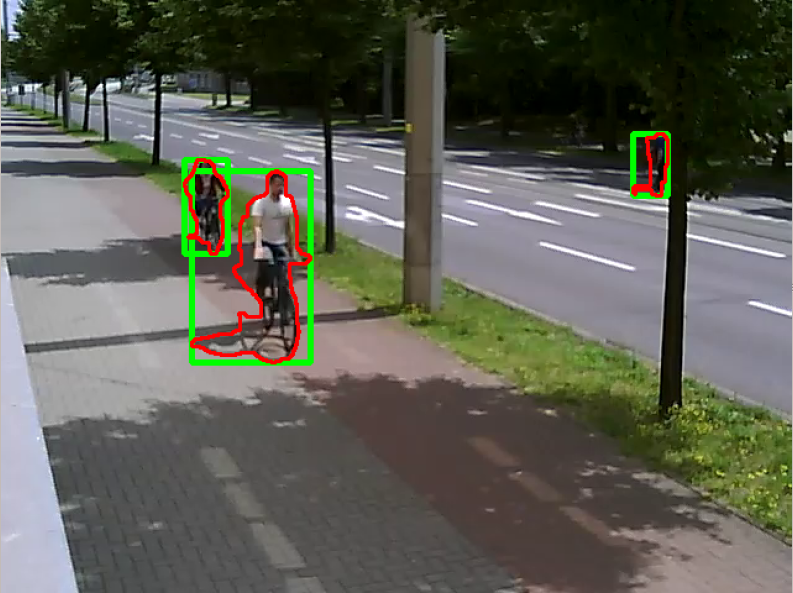
\includegraphics[width=0.5\textwidth]{ds10_contour}
\caption{Erfolgreiche Segmentierung bei schwierigen Verhältnissen}
\end{figure}

\subsubsection{Backgroundsubstraction}
Für die Bewegungssegmentierung nutzen wir den von OpenCV bereitgestellten \textit{BackgroundSubstractorMOG2}, der das Gaussian Mixture Model (GMM) nach dem Verfahren von Z. Zivkovic \cite{zivkovic} benutzt. Dabei verzichten wir jedoch auf die eingebaute Schattensegmentierung, da diese nicht zuverlässig genug für uns ist. Der Backgroundsubstractor erstellt aus den letzten \textit{k} Frames mit HIlfe von GMM ein Hintergrundbild. Zwischen diesem und dem aktuellen Frame wird ein Differenzbild erstellt. In diesem Differenzbild sind Bereiche in denen sich nichts bewegt hat dunkel und Bereiche in denen eine Bewegung stattgefunden hat, sind hell. Durch eine Schwellenwertoperation erhält man so eine Maske, welche die bewegten Objekte segmentiert. Das Ergebnis ist in Abbildung \ref{fig:foreground} zu sehen.
Durch empirische Untersuchung haben sich folgende Parametereinstellungen als zufriedenstellend erwiesen:
\begin{itemize}
	\item nmixtures = 10
	\item backgroundRatio = 0.9
	\item history = 45
	\item varThresholdGen = 55
	\item varThreshold = 4
\end{itemize}
Um das Rauschen in der erstellten Maske zu unterdrücken filtern wir diese durch einen Medianfilter mit geringer Kernelgröße. Bei der Backgroundsubstraction kann es vorkommen, dass nur Teile von einem Objekt segmentiert werden, die jedoch sehr nahe an einander liegen. Diese verbinden wir durch ein morphologisches closing.
Damit wir nun aus der Maske einzelne Objekte erhalten, führen wir eine Connected Componend Analyse mittels der OpenCV-Funktion \textit{findContours} aus. Objekte die eine bestimmte Mindestgröße unterschreiten werden dabei entfernt, da diese als irrelevant zu erachten sind.


\begin{figure}
\centering
\begin{subfigure}[t]{.23\textwidth}
\centering
%\setlength{\abovecaptionskip}{15pt plus 5pt minus 10pt}
  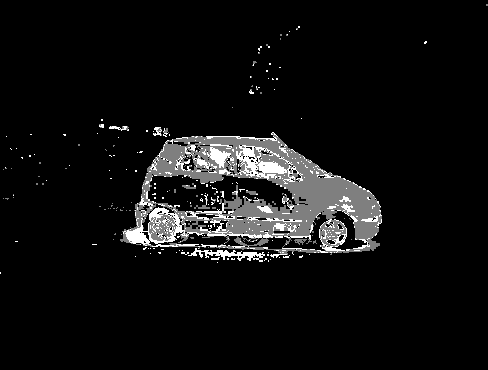
\includegraphics[width=1\linewidth]{trainds01_foregroundmask}
  \caption{Vordergrundmaske, grau stellt den detektierten Schatten dar}
  \label{fig:sub1}
\end{subfigure}
\begin{subfigure}[t]{.23\textwidth}
\centering
%\setlength{\abovecaptionskip}{25pt plus 15pt minus 15pt}
  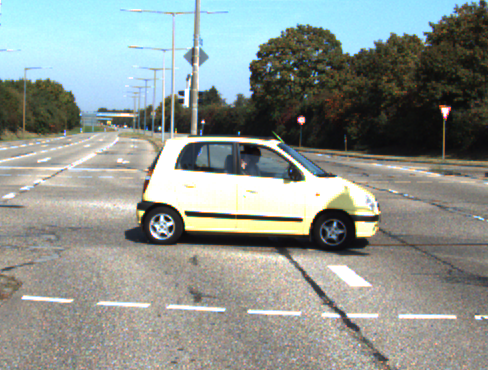
\includegraphics[width=1\linewidth]{trainds01_original}
  \caption{Originalbild}
  \label{fig:sub2}
\end{subfigure}
\caption{Ergebnis der Backgroundsubstraction}
\label{fig:test}
\end{figure}

\subsubsection{Nachverarbeitung}
Um das Problem von Teilverdeckungen zu beheben, haben wir einen einfachen Nachverarbeitungsschritt entwickelt, der ähnliche Aufgaben, wie ein aufwändigeres Tracken übernehmen soll. Dazu gehen wir davon aus, dass wir im vorherigen Frame ein Objekt \textit{A} mit der bounding Box \textit{b} detektiert haben. Im aktuellen Frame wird dann in einem Bereich \textit{b'=s*b} nach neu detektierten Objekten gesucht. Dabei ist \textit{s} ein non-uniformer Skalierungsfaktor, der in der Horizontalen größer ist, als in der Vertikalen, da wir davon ausgehen, dass sich die Objekte schneller in horizontaler, als in vertikaler Richtung bewegen. Liegt die bounding Box von einem oder mehreren neu detektierten Objekten komplett innerhalb von \textit{b'}, dann werden diese einem Gesamtobjekt zugeordnet, wie in Abbildung \ref{fig:trainds01_nachverarbeitung} zu sehen. Dabei bleiben die erkannten Konturen erhalten, nur die bounding Boxes werden vereinigt. Durch diese Neugruppierung kann es passieren, dass sich gruppierte Objekte über das gesamte Bild ausdehnen, daher wird eine Gruppierung aufglöst, sobald die gruppierten Objekte sich zu weit von einander entfernen. Die so entstandenen Objekte werden im Folgenden an den Klassifikator weiter gereicht.

\begin{figure}
\centering
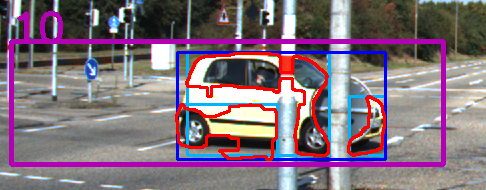
\includegraphics[width=0.5\textwidth]{./trainds01_nachverarbeitung}
\caption{in Lila ist der Suchbereich b' zu sehen, hellblau sind die bounding Boxes der neu detektierten Konturen, dunkelblau ist das gruppierte Obkjekt}
\label{fig:trainds01_nachverarbeitung}
\end{figure}

\subsection{Klassifikation}

\begin{figure*}
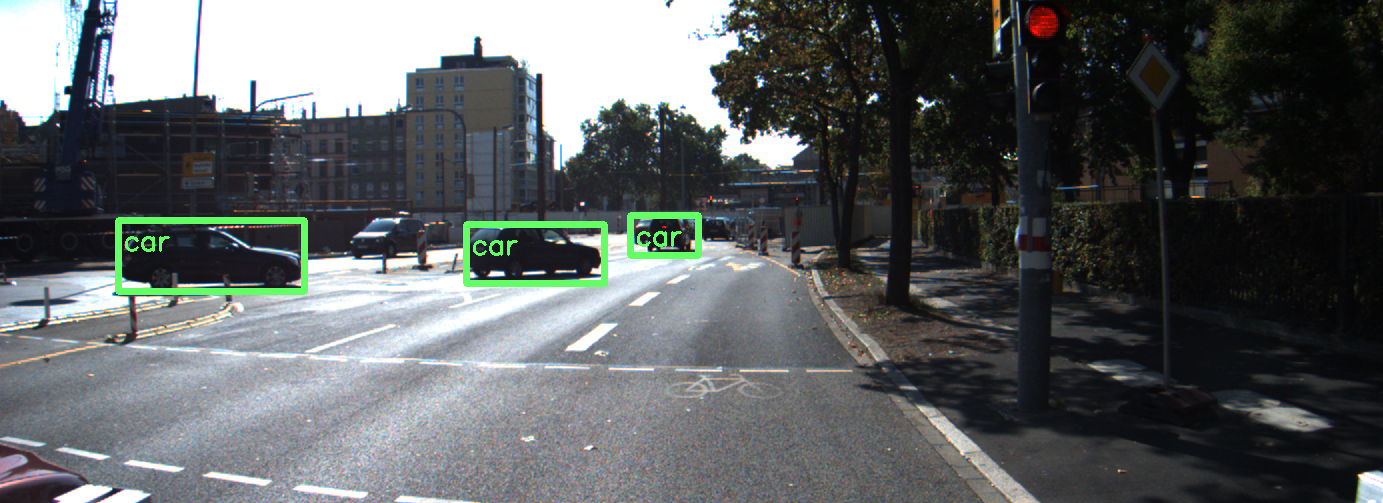
\includegraphics[width=\textwidth]{ds03_car01}
\caption{Ergebnis der Klassifikation auf mehreren ROI}
\end{figure*}

\subsubsection{Haar-Feature-Cascade-Classifier}

Die Klassifikation ist über einen Haar-Feature-Cascade-Classifier implementiert.
Dafür wird für jede Klasse eine eigens trainierte Klassifikationsdatei im XML-Format benötigt. Da wir die Klassen \textit{Auto}, \textit{Mensch} und \textit{Fahrrad} unterscheiden wollen benötigen wir drei Klassifikationsdateien. Diese XML-Dateien werden bei Programmstart geladen und teilen dem Klassifikator die Parameter mit, auf die er reagieren soll. Anschließend können wir den Klassifikator auf eine beliebige Region-Of-Interest (ROI) anwenden. Als Ergebnis erhalten wir eine Liste von Bereichen innerhalb der ROI mit erkannten Objekten. Somit bekommen wir unter anderem ein binäres Ergebnis - \textit{gefunden} wenn die Liste mindestens einen Eintrag hat oder \textit{nicht gefunden} wenn die Liste leer ist. Der Vorteil an dieser Methode liegt darin, dass wir somit mehrere Objekte innerhalb einer gegebenen ROI erkennen können. Wenn wir uns allerdings sicher sind, dass die gegebene ROI nur ein Objekt enthalten kann, fällen wir das Urteil anhand der Schwierigkeit der Detektion der Klasse und Anzahl der gefundenen Bereiche. Somit entscheiden wir uns für die Klasse Fahrrad, sobald der Klassifikator mindestens ein Fahrrad gefunden hat, da dies für unseren Klassifikator die am schwierigsten zu detektierende Klasse ist. Dass auf den meisten Fahrrädern Menschen sitzen ist ein weiterer Grund die Klassifikation nach Menschen erst durchzuführen, wenn kein Fahrrad erkannt wurde.
Wenn kein Fahhrad in der ROI gefunden wurde, wird anschließend nach Menschen gesucht und zuletzt nach Autos.


\subsubsection{Training}

Da das Erzeugen einer Klassifikationsdatei je nach Schwierigkeit und gewünschter Genauigkeit mehrere Stunden bis Tage dauern kann, wurde nach bereits verfügbaren, trainierten Klassfikationsdateien gesucht um den Aufwand in einem vertretbaren Rahmen zu halten. Fündig wurden wir allerdings nur in den OpenCV-Beispielen mit dem \textit{haarcascade\_mcs\_upperbody.xml} als robusten Klassifikator für Menschen. 

Die Klassifikationsdateien für Fahrräder und Autos mussten wir selbst erstellen.
Dazu haben wir uns im wesentlichen an eine Anleitung\cite{Seo:Haartraining} von \textit{Naotoshi Seo} gehalten. In dieser wurden die folgenden Schritte beschrieben:
\begin{itemize}
	\item Vorbereitung der Daten
	\item Samples erzeugen
	\item Training
\end{itemize}
Zusätzlich hat der Autor mit \textit{mergevec.cpp} und \textit{createtrainsamples.pl} zwei kleine Programme veröffentlicht, mit denen man sehr schnell Datensätze für Positiv- und Negativbilder erzeugen kann. Die so erzeugten Datensätze werden wiederum an das Programm \textit{opencv\_haartraining} gegeben, zusammen mit Parametern die im wesentlichen die Qualität und Laufzeit des Trainings bestimmen.
Für das Training der Klassifikationsdatei für Autos haben wir ausschließlich Positivbilder aus den gegebenen Testdaten erzeugt. Für die Fahrräder haben wir zusätzlich zu den gegebenen Testdaten noch Fahrradbilder aus einem frei verfügbaren Datensatz\cite{Caltech256} als zusätzliche Positivbilder genutzt. In beiden Fällen wurde der Datensatz der Negativbilder aus einer größeren Bildersammlung sowie den Positivbildern der jeweils anderen Klassen erstellt.

\subsubsection{Nachverarbeitung}
In einem weiteren Nachverarbeitungsschritt wird für jedes klassifizierte Objekt im aktuellen Frame geprüft, wie oft es in vergangenen Frames als welche Klasse klassifiziert wurde. Wenn ein Objekt \textit{O} mehr als \textit{X} mal einer bestimmten Klasse \textit{C} zugewiesen wurde und es den anderen Klassen weniger oft zugewiesen wurde, dann wird das Objekt \textit{O} der Klasse \textit{C} zugewiesen, auch wenn es im aktuellen Frame anders klassifiziert wurde.

\section{Verworfene Bestandteile}
Im laufe des Projektes wurden viele Verfahren getestet, um das Ziel zu erreichen. Die bisher beschriebenen haben sich dabei als am besten geeignet herausgestellt. In diesem Abschnitt möchten wir darauf eingehen, welche weiteren Verfahren getestet und danach wieder verworfen wurden und warum wir sie verworfen haben.

\subsection{Optischer Fluss}
Mit Hilfe eines dichten optischen Flusses, hatten wir uns erhofft sowohl die Segmentierung, als auch Teile des Trackens zu erledigen. Wir haben dazu mit der von OpenCV bereitgestellten Funktion \textit{calcOpticalFlowFarneback} experimentiert, jedoch keine passenden Parameter gefunden, die akzeptable Ergebnisse liefern. Da wir zu diesem Zeitpunkt bereits brauchbare Ergebnisse mit der Backgroundsubstraction erziehlt hatten, haben wir beschlossen unsere Zeit in die Verfeinerung dieses Verfahrens, sowie die Klassifizierung zu investieren. 
\subsection{Tracking durch SURF}
Als weiteren Ansatz zum Tracken haben wir mit SURF (Speeded Up Robust Features) experimentiert um in einem Frame erkannte Objekte im nächsten Frame wieder zu finden. Dabei werden Features des erkannten Objektes und deren relative Position zueinander im vorherigen Frame extrahiert und versucht im aktuellen Frame in ähnlicher Anordnung wiederzufinden. Dies hat auch akzeptable Ergebnisse für Autos geliefert, da sich bei diesen die Features von Frame zu Frame nicht zu stark ändern. Bei Fußgängern und Radfahrern hingegen schlug dieser Ansatz komplett fehl, weshalb er wieder verworfen wurde.

\subsection{Klassifikation anhand einfacher Merkmale}

Zu Anfang der Projektarbeit war uns der Gedanke gekommen, dass es recht elegant wäre auf komplizierte, zu trainierende Klassifikatoren zu verzichten und stattdessen lieber einen einfacheren und nachvollziehbaren Ansatz zu verfolgen: Klassifikation anhand von Seitenverhältnis und markanten Linien. Hintergrundgedanke war, dass die Kamera in den meisten Fällen einen kleinen Horizontalwinkel haben wird, so dass der Horizont - falls sichtbar - eine nahezu horizontale Linie auf dem Bild abbilden würde. Basierend auf dieser Annahme wären Menschen die laufen höher als breit. Autos dagegen breiter als hoch. Fahrradfahrer wären ähnlich der Autos breiter als hoch. Hier hätten die Linienkomponenten helfen sollen. Eine weitere Idee war mittels Template Matching die Reifen zu extrahieren und anhand von deren Größenverhältnis zum gesamten Objekt zwischen Fahrrad und Auto zu unterscheiden.
Da wir uns mit der Linienkomponente nicht sehr sicher waren, die Detektion von sich auf die Kamera zu- und wegbewegenden Fahrrädern und Autos nicht in unser Konzept gepasst haben und wir nicht so viel Zeit zum herumexperimentieren hatten, entschieden wir uns für einen \textit{klassischen} Ansatz der mit gewisser Sicherheit zu einem soliden Ergebnis führen sollte.



\section{Evaluierung}

Die Evaluierung zeigt ein durchwachsenes Bild.
Unser Ansatz hat auf den Datensätzen 3 bis 7 und 13 gut bis sehr gut funktioniert. Auf den restlichen Datensätzen hat unser Verfahren mittelgute bis schlechte Ergebnisse erzielt. Generell hat sich gezeigt, dass die Segmentierung meist gut bis sehr gut funktioniert, die Klassifkation dagegen nicht so robust ist.
Vor allem wenn sich die Art des Datensatzes stark von den Trainingsdatensätzen unterscheidet, fallen starke Mängel in der Klassifikation auf. Bei den Testdatensätzen 8 bis 12 zeigt sich beispielsweise, dass der Klassifkator mit den Kamerapositionen nicht klarkommt, da mit keinen Positivbildern aus diesen Perspektiven trainiert wurde und somit der Klassifikator nur wenig Chancen hat, seine Arbeit erfolgreich zu erledigen.
Andererseits zeigte sich, dass unser Verfahren sehr schnell ist und wir je nach Datensatz ein bis mehrere Bilder pro Sekunde mit der kompletten Pipeline an Berechnungen erhalten.

\begin{figure}
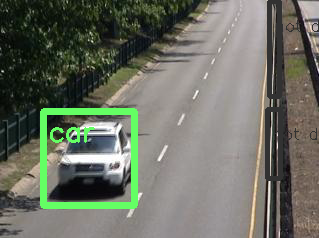
\includegraphics[width=0.5\textwidth]{ds13_car01}
\caption{Erfolgreiche Klassifikation mit Fehlsegmentierung}
\end{figure}

\section{Schluss}

Wir haben es geschafft mit einfachen Mitteln einen verhältnismäßig schnellen Algorithmus mit Hilfe der OpenCV-Bibliothek zu erstellen. Dieser arbeitet auf günstigen Datensätzen zuverlässig mit einer guten Detektionsrate. Bei schwierigeren Datensätzen zeigt unser Ansatz allerdings Schwächen.

\subsection{Ausblick}
Mit besser trainierten Daten und einem Austausch der Ergebnisse zwischen Klassifikator und Segmentierungsroutine wären deutlich bessere Ergebnisse erzielbar.
Für perfekte Ergebnisse müssten allerdings die Algorithmen umgestellt werden. Je nach einsetzbarem Rechenaufwand pro Bild könnte man robustere Verfahren nutzen, sowohl für die Segmentierung und Objektverfolgung, als auch die Klassifikation. So wäre beispielsweise eine Median-basierte Hintergrundbilderzeugung ein Grundstein für eine robustere Segmentierung, würde allerdings gleichzeitig einen enorm höheren Rechenaufwand benötigen.
Außerdem könnte man die Segmentierten Konturen tracken um so plötzliche Veränderungen der Kontur einzuschränken.
Bei der Klassifikation müsste man für unterschiedliche Klassen unterschiedliche Verfahren nutzen. Für Autos könnte man das aktuelle Verfahren, d.h. den Haar-Feature-Cascade-Classifier beibehalten. Für Menschen und Fahrräder könnte man beispielsweise auf einen HOG-Cascade-Classifier wechseln um bessere Ergebnisse zu erzielen.
Zusätzlich sollte man - wie bereits erwähnt - die Ergebnisse von Klassifikator und Segmentierungsroutine ineinander einfließen lassen. So könnte man zu Beginn einer Sequenz die Klassifikatoren auf dem gesamten Bild nach potentiellen Objekten suchen lassen. Anschließend merkt man sich diese Region-Of-Interests für potentielle Bewegungen vor. Weiterhin könnte man bei getrackten Objekten die Klassifikation robuster gestalten, indem man sich für ein Objekt die detektierte Klasse merkt und einen sprunghaften Wechsel der Klasse von getrackten Objekten verhindert.


\begin{figure}
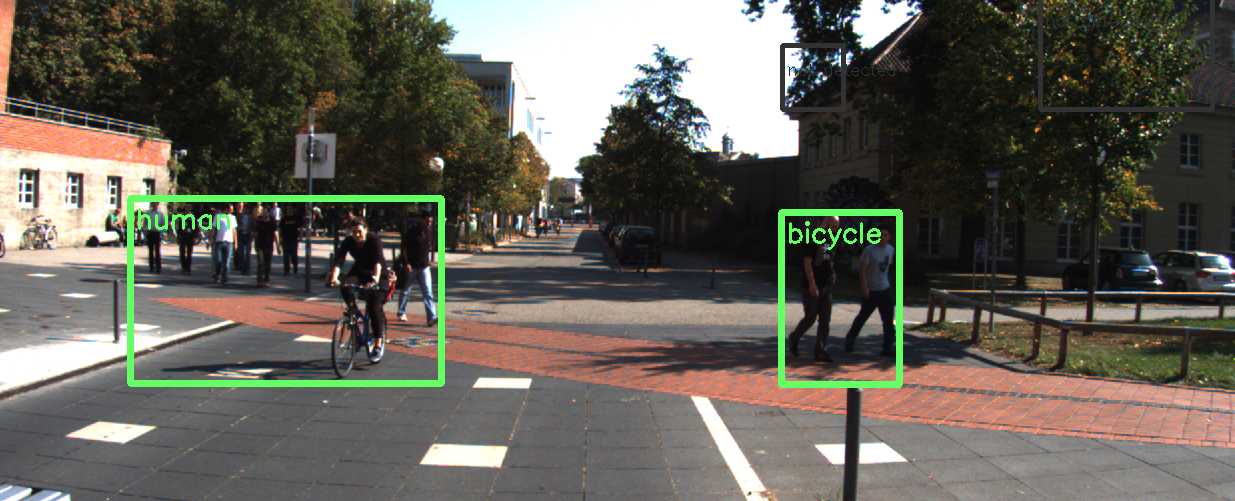
\includegraphics[width=0.5\textwidth]{ds06_failed}
\caption{Fehlerhafte Klassifikation}
\end{figure}


% conference papers do not normally have an appendix


% use section* for acknowledgement
%\section*{Acknowledgment}
% The authors would like to thank...





% trigger a \newpage just before the given reference
% number - used to balance the columns on the last page
% adjust value as needed - may need to be readjusted if
% the document is modified later
%\IEEEtriggeratref{8}
% The "triggered" command can be changed if desired:
%\IEEEtriggercmd{\enlargethispage{-5in}}

% references section

% can use a liography generated by BibTeX as a .bbl file
% BibTeX documentation can be easily obtained at:
% http://www.ctan.org/tex-archive/biblio/bibtex/contrib/doc/
% The IEEEtran BibTeX style support page is at:
% http://www.michaelshell.org/tex/ieeetran/bibtex/
%\bibliographystyle{IEEEtran}
% argument is your BibTeX string definitions and bibliography database(s)
%\bibliography{IEEEabrv,../bib/paper}
%
% <OR> manually copy in the resultant .bbl file
% set second argument of \begin to the number of references
% (used to reserve space for the reference number labels box)
\renewcommand*{\refname}{Quellen}
\begin{thebibliography}{1}
	\bibitem{opencv}
		\url{http://opencv.org/}
	\bibitem{cmake}
		\url{http://cmake.org/}
	\bibitem{git}
		\url{http://git-scm.com/}
	\bibitem{github}
		\url{https://github.com/polybos/cv-project}
	\bibitem{zivkovic}
		Z.Zivkovic, Improved adaptive Gausian mixture model for background subtraction
	\bibitem{Seo:Haartraining}
		\url{http://note.sonots.com/SciSoftware/haartraining.html}
	\bibitem{Caltech256}
		\url{http://www.vision.caltech.edu/Image_Datasets/Caltech256}
\end{thebibliography}




% that's all folks
\end{document}


